%8.9.03

\chapter{Euler-Charakteristik}
\label{sec:Euler}

F"ur die Anzahl der Ecken $e$, die der Kanten $k$ und die der Fl"achen $f$ eines W"urfels gilt $e-k+f=2$. Teilt man eine Fl\"ache des W\"urfels, entstehen neue Ecken oder Kanten, die den Beitrag der zus\"atzlichen Fl\"ache wegheben, und es gilt weiterhin $e-k+f=2$. Der Eulerschen Polyedersatz besagt, dass diese Beziehung f"ur alle konvexen Polyeder $P$ gilt \cite{Saskin:89}. F\"ur eine Figur $F$, die nur aus Fl\"achen, Kanten und Ecken besteht, definiert man die Euler-Charakteristik durch
\begin{equation}
  \chi(F):=e-f+k.
\end{equation}
Die Euler-Charakteristik ist unabh\"angig von der Zerlegung und daher eine topologische Invariante von $F$. Deformiert  man $F$, bleibt $\chi(F)$ konstant. Es gibt eine Reihe von M\"oglichkeiten, die Euler-Charakteristik einer gegebenen Figur auszurechnen. Im ersten Teil des Kapitels werden die Facetten von $\chi$, die f\"ur diese Arbeit relevant sind, vorgestellt. Der zweite Teil besch\"aftigt sich mit Methoden, die Euler-Charakteristik von Gitterclustern auszurechnen.

\section{Euler-Charakteristik auf dem Konvexring}
Die Euler-Charakteristik wurde von Hadwinger \cite{Hadwinger:57} axiomatisch f\"ur alle endlichen Vereinigungen und Durchschnitte konvexer K\"orper eingef\"uhrt.
Ein $d$-dimensionaler konvexer K\"orper ist eine kompakte, d.h. beschr\"ankte und abgeschlossene, konvexe Teilmenge des $\mathbb{R}^d$, die in keiner nieder-dimensionalen affinen Hyperebene enthalten ist. Man definiert f\"ur alle konvexen K\"orper $A$ die Euler-Charakteristik durch $\chi(A):=1$ und f\"ur die leere Menge durch $\chi(\emptyset):=0$. Da der Durchschnitt zweier konvexer K\"orper wiederum ein konvexer K\"orper ist, kann kann die Euler-Charakeristik mit der Definition 
\begin{equation}
  \label{eq:additivity}
\chi(A\cup B):=\chi(A)+\chi(B)-\chi(A \cap B)
\end{equation}
auf Vereinigungen von konvexen K\"orpern, die im Allgemeinen nicht konvex sind, ausgedehnt werden. Die Menge aller endlichen Vereinigungen und Durchschnitte konvexer K\"orper ist unter weiteren Vereinigungen und Schnitten abgeschlossen und bildet den Konvexring $\mathcal{K}$. Durch (\ref{eq:additivity}) ist $\chi$ auf dem gesamten Konvexring definiert. Die so definierte Euler-Charakteristik ist immer eine ganze Zahl und bleibt deshalb bei kontinuierlichen Deformationen der K\"orper konstant. Der Rand $\partial A$ eines $d$-dimensionalen konvexen K\"orpers $A$ ist homotop zu einer $(d-1)$-Sph\"are und es gilt $\chi(\partial A)=0$ falls $d$ gerade und $\chi(\partial A)=2$ falls $d$ ungerade ist.\\
F\"ur eine Vereinigung von konvexen K\"orpern $X=\cup_{i} A_i$ folgt durch Induktion aus (\ref{eq:additivity})
\begin{equation}
\label{eq:induction}
\chi(X) =  \chi\left(\bigcup_i A_i\right)=\sum_i \chi(A_i)-\sum_{i<j} \chi (A_i\cap A_j)  + \sum_{i< j < k}\chi(A_i \cap A_j \cap A_k)- \cdots. 
\end{equation}
Am Beispiel des Randes $\partial W$ eines W\"urfels $W$ soll die axiomatische Definition der Euler-Charakteristik erl\"autert werden. Der Rand eines W\"urfels ist die Vereinigung seiner sechs Fl\"achen $\cup_{i=1}^6 F_i$. Wendet man Gleichung (\ref{eq:induction}) auf $\partial W$ an, so k\"onnen die einzelnen Summen den Fl\"achen, Kanten und Ecken zugeordnet werden.  Die erste Summe ist die Anzahl der Fl\"achen $f$, denn $\chi(F_i)$ ist $1$. Der Durchschnitt zweier Fl\"achen ist entweder leer oder eine Kante, deren Euler-Charakteristik $1$ ist. Daher ist die zweite Summe gleich der Zahl der Kanten. Entsprechend ist der Durchschnitt dreier Fl\"achen entweder eine Ecke oder leer, und die dritte Summe ist gleich der Zahl der Ecken. Der Durchschnitt von mehr als drei Fl\"achen ist leer. F\"ur den Rand eines W\"urfels stimmt die Euler-Charakteristik auf dem Konvexring also mit $\chi(\partial W)=e-k+f$ \"uberein. Die Berechnung der Euler-Charakteristik mit Gleichung (\ref{eq:induction}) wird aber sehr aufwendig, wenn viele der $A_i$ einen nichtleeren Durchschnitt haben.
\\Die Euler-Charakteristik einer beliebigen Figur, die eine Zerlegung in konvexe Zellen (Ecken, Kanten, Fl\"achen, Polyeder und deren h\"oherdimensionale Analoga) zul\"asst, ist die alternierende Summe $\sum_{k=0}^d (-1)^k \lambda_k$ der Anzahl $k$-dimensionaler Zellen $\lambda_k$ \cite{Saskin:89}. Es ist zweckm\"a"sig, die Figur als disjunkte Vereinigung der Zellen ohne ihren Rand zu betrachten und f\"ur konvexe $k$-dimensionale Zellen ohne Rand $\chi(\check{K})=(-1)^k$ mit  $\check{K}=K\backslash \partial K$ zu definieren. Die Euler-Charakteristik ist dann einfach die Summe der Beitr\"age der randlosen Zellen. Randlose $k$-dimensionale Zellen sind offene Teilmengen einer $k$-dimensionalen Hyperebene.


\section{Euler-Charakteristik und Gau"s'sche Kr\"ummung}
\label{sec:Gauss}
Falls ein K\"orper einen hinreichend glatten Rand hat, stiftet ein verallgemeinertes Gau"s-Bonnet-Theorem einen Zusammenhang zwischen der topologischen Invariante $\chi$ und dem Oberf\"achenintegral der Gau"s'schen Kr\"ummung. 
\\Die Oberfl\"ache $\partial X$ eines hinreichend glatten $d$-dimensionalen Gebiets $X$ ist eine kompakte, orientierbare, $(d-1)$-dimensionale Mannigfaltigkeit ohne Rand (der Rand eines Randes ist $\emptyset$) in $\mathbb{R}^d$. Die Orientierung wird durch den nach au"sen gerichteten Normalenvektor $\mathbf{n}(x)$ gegeben. Die Gau"s'sche Kr\"ummung $\kappa(x)$ ist die Jacobi-Determinante der Gau"sabbildung $g:\partial X \rightarrow S^{d-1}$ mit $g(x)=\mathbf{n}(x)$. F\"ur eine kompaktes glattes Gebiet $X$ im $\mathbb{R}^d$ gilt, dass der Grad der Gau"sabbildung auf $\partial X$ gleich der Euler-Charakteristik von $X$ ist (siehe das Buch von Bredon  \cite{Bredon:93}, Abschnitt VI, Theorem 12.11). 
\begin{equation}
  \label{eq:curvature}
 \chi(X)=deg(g)=\frac{1}{\omega_{d-1}}\int_{\partial X} \kappa(x) d\mathcal{O},
\end{equation}
wobei $\omega_{d-1}$ die Oberfl\"ache der Einheitssph\"are $\mathbb{S}^{d-1}$ und $deg(g)$ der Grad der Gau"sabbildung $g$ ist. Der Grad einer Abbildung gibt, grob gesagt, an, wie oft das Bild der Abbildung die Sph\"are $S^{d-1}$ \"uberdeckt. \\
Ist $d$ ungerade, gilt f\"ur $\partial X$ das klassische Gau"s-Bonnet-Theorem    
\begin{equation}
  \chi(\partial X)=\frac{2}{\omega_{d-1}}\int_{\partial X} \kappa(x) d\mathcal{O}
\end{equation}
und damit $\chi(\partial X)=2\chi(X)$. F\"ur gerade $d$ ist $\chi(\partial X)=0$. 
\\F\"ur sp\"atere Anwendungen ist es sinnvoll die Euler-Charakteristik auch f\"ur K\"orper, die ihren Rand nicht enthalten, zu definieren, wie dies f\"ur konvexe Zellen schon angedeutet wurde. Dies geschieht unter Ausn\"utzung der Additivit\"at von $\chi$ durch 
\begin{equation}
\label{eq:opensets}
\chi(X \backslash \partial X):=\chi(X)-\chi(\partial X)=(-1)^{d+1}\chi(X).
\end{equation}
Eine solche Definition der Euler-Charakteristik f\"ur offene Mengen kann problematisch sein, f\"uhrt bei umsichtiger Anwendung aber auf keine Schwierigkeiten.\\ 

Der Zusammenhang zwischen integraler Oberfl\"achenkr\"ummung und der Euler-Charak"-ter"-istik kann auch \"uber den Steinerschen Satz aus der Integralgeometrie erhalten werden. F\"ur konvexe K\"orper l\"asst sich das Parallelvolumen durch Integrale \"uber elementarsymmetrische Funktionen der Hauptkr\"ummungen ausgedr\"ucken. \"Uber den Steinerschen Satz werden die Minkowski-Funktionale, darunter die Euler-Charakteristik, mit den Kr\"ummungsintegralen durch Koeffizientenvergleich identifiziert. Durch die Additivit\"at lassen sich die so gewonnenen Beziehungen auf den Konvexring ausdehnen (siehe \cite{Santalo:76} oder \cite{Mecke:94}).\\
Die Oberfl\"achenkr\"ummung eines Polyeders im $\mathbb{R}^3$ ist in den Ecken ``konzentriert''. Den Normalenvektoren der eine Ecke umgebenden Fl\"achen entsprechen Punkte auf der Sph\"are. Verbindet man diese Punkte mit Gro"skreisen, entspricht die eingeschlossene Fl\"ache der Gau"sschen Kr\"ummung dieser Ecke. Abh\"angig vom Umlaufsinn und der Umlaufzahl wird der Beitrag negativ oder positiv und mit unterschiedlicher Multiplizit\"at gez\"ahlt. Summation \"uber die Beitr\"age aller Ecken liefert das Gau"s-Bonnet-Theorem f\"ur Polyeder in drei Dimensionen (siehe Banchoff \cite{Banchoff:70}).   

\section{Morsetheorie}
Auf einem $d$-dimensionalen K\"orper $X$, der im $\mathbb{R}^d$ eingebettet ist, l\"asst sich durch den Abstand $r(x)$ eines Punktes $x\in X$ von einer Hyperebene $H$ eine H\"ohenfunktion definieren. Hat der K\"orper einen hinreichend glatten Rand, so ist $h(x)=r(x)|_{x\in \partial X}$ in geeigneter Parametrisierung zweimal stetig differenzierbar. $h(x)$ hat mindestens zwei kritische Punkte, in denen $\nabla h$ verschwindet. In drei Dimensionen entsprechen diesen kritischen Punkten die Minima, Maxima und Sattelpunkte. Wenn die Hessematrix der H\"ohenfunktion $\left(H_{ij}\right)=\left(\frac{\partial^2 h}{\partial x_i \partial x_j}\right)$ an den kritischen Punkten nicht singul\"ar ist, heisst $h(x)$ Morsefunktion. Die Morsezahl $m_\lambda$ ist die Anzahl derjenigen kritischen Punkte, deren Hessematrix $\lambda$ negative Eigenwerte hat. Nach dem Morsetheorem \cite{Milnor:68} gilt, dass die alternierende Summe $\sum_{\lambda=0}^{d-1} (-1)^\lambda m_\lambda$ gleich der alternierenden Summe der Betti-Zahlen von $\partial X$ und damit gleich der Euler-Charakteristik $\chi(\partial X)$ ist.\\
Auch das Morsetheorem kann, ganz analog zum Gau"s-Bonnet-Theorem, auf Polyeder in drei Dimensionen verallgemeinert werden. Die kritischen Punkte sind gerade die Ecken des Polyeders. Man w\"ahlt einen Vektor $\mathbf{n}$, der auf keiner Fl\"ache oder Kante des Polyeders senkrecht steht. Um den Index einer Ecke $e$ zu bestimmen, betrachtet man einen kleinen Kreis um $e$, der in einer Ebene mit Normalenvektor $\mathbf{n}$ liegt. Die Zahl $c(e)$ der Schnittpunkte des Kreises mit dem Polyeder liefert \"uber $i(e)=1-\frac{c(e)}{2}$ den Index der Ecke. Summation der Indices aller Ecken ergibt $\chi$ (siehe Banchoff \cite{Banchoff:70}). 

\subsection{Schnittrekursion}
Die Schnittrekursion ist ein eng mit der Morsetheorie verwandtes Verfahren, die Euler-Charakteristik auszurechnen. Sei ein K\"orper $X$ mit Rand $\partial X$ gegeben. Statt einer H\"ohenfunktion $h_{\mathbf{n}}$ auf $\partial X$ betrachtet man eine Schar von Hyperebenen $E_r$ mit Normalenvektor $\mathbf{n}$ und Abstand $r$ vom Ursprung. Die Euler-Charakteristik des Schnitts von $E_r$ mit $X$ \"andert sich mit $r$ nur, wenn ein kritischer Punkt der entsprechenden H\"ohenfunktion $h_{\mathbf{n}}$ auf $\partial X$ in $E_r$ liegt. Die \"Anderung von $\chi(E_{r}\cap X)$ ist abh\"angig vom Index des kritischen Punktes. Die Euler-Charakteristik $\chi(X)$ ergibt sich durch Summation \"uber die \"Anderungen von $\chi(E_{r}\cap X)$ an allen Werte $r_c$, an denen kritische Punkte von $h_{\mathbf{n}}$ liegen:
\begin{equation}
  \chi(X)=\sum_{r_c} \chi(E_{r_c}\cap X)-\lim_{\epsilon \rightarrow 0}\chi(E_{r_c+\epsilon}\cap X).
\end{equation}
Dadurch kann die Berechnung der Euler-Charakteristik rekursiv auf Schnitte in immer kleineren Dimensionen zur\"uckgef\"uhrt werden. Eine Herleitung f\"ur $X$ aus dem Konvexring ist in \cite{Hadwinger:55} gegeben. F\"ur ein-, zwei- und dreidimensionale Systeme ist das Verfahren leicht einzusehen und soll hier kurz vorgef\"uhrt werden.\\
In einer Dimension ist $X$ eine abgeschlossenes Intervall $[a,b]$ der reellen Zahlen. Die Endpunkte des Intervalls sind die kritischen Punkte, und eine Hyperebene besteht aus einem Punkt. Die Schnittrekursion (siehe Abb. \ref{fig:morse1d}) liefert das triviale Ergebnis $\chi(X)=1$. 
\begin{figure}[bp]
  \centering
  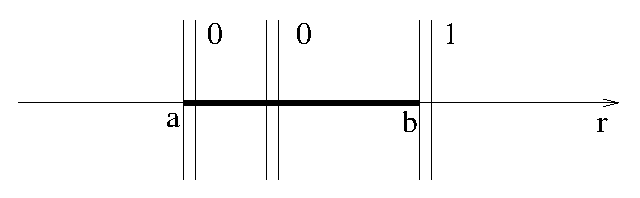
\includegraphics{./Euler-figs/morse1d}
  \caption{Schnittrekursion in einer Dimension. Nur der Punkt $r=b$ liefert einen Beitrag.}
  \label{fig:morse1d}
\end{figure}
Die Euler-Charakteristik einer eindimensionalen Figur ist daher die Zahl der Komponenten der Figur.  
\\In zwei Dimensionen sind kritische Punkte von $h_{\mathbf{n}}$ nach oben oder unten ausgerichtete Kuppen oder Mulden (siehe Abb. \ref{fig:2dschnitt}). Bei nach unten ausgerichteten Mulden oder Kuppen \"andert sich die $\chi(E_{r}\cap X)$ nicht, bei nach oben ausgerichteten Kuppen ist $\chi(E_{r_c}\cap X)-\lim_{\epsilon \rightarrow 0}\chi(E_{r_c+\epsilon}\cap X)=1$ und bei nach oben ausgerichteten Mulden ist $\chi(E_{r_c}\cap X)-\lim_{\epsilon \rightarrow 0}\chi(E_{r_c+\epsilon}\cap X)=-1$. F\"ur den \"au"seren Rand ergibt sich dadurch ein Beitrag $+1$, f\"ur alle inneren R\"ander $-1$. 
In zwei Dimensionen ist $\chi(X)$ also die Zahl der Komponenten von $X$, abz\"uglich der Zahl der L\"ocher in diesen Komponenten.
\begin{figure}[htbp]
  \centering
  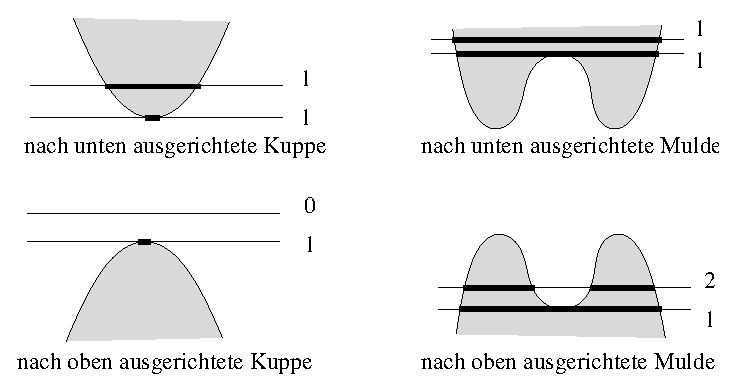
\includegraphics{./Euler-figs/2dschnitt}
  \caption{Schnittrekursion in zwei Dimensionen.}
  \label{fig:2dschnitt}
\end{figure}
\\In drei Dimensionen muss zwischen Maxima, Minima und Sattelpunkten unterschieden werden. Man \"uberlegt sich einfach, dass Maxima und Minima in bestimmten Orientierungen einen Beitrag $+1$ liefern, w\"ahrend Sattelpunkte $-1$ beitragen. Die Euler-Charakteristik in drei Dimensionen ist daher die Zahl der Komponenten, abz\"uglich der Zahl der Tunnel oder Henkel, plus der Zahl der Einschl\"usse.\\
Die Punkte, an denen sich $\chi(E_{r}\cap X)$ \"andert, lassen sich auch ohne eine differenzierbare H\"ohenfunktion angeben, und ein glatter Rand von $K$ ist f\"ur die Anwendbarkeit der Schnittrekursion nicht notwendig. Deshalb ist die Schnittrekursion f\"ur die Anwendung auf Gittern besonders geeignet.

\section{Euler-Charakteristik in der Graphentheorie}
\label{sec:graphen}
Hier sollen einige Begriffe der Graphentheorie erw\"ahnt werden, auf die im weiteren Verlauf zur\"uckgegriffen wird. Eine umfangreiche Sammlung von Definitionen der Begriffe der Graphentheorie ist in \cite{Essam:70} zu finden. \\
Ein \textit{Graph} $G$ besteht aus einer Vertexmenge $V$ und einer Kantenmenge $E$, die ungeordnete Paare von Vertices enth\"alt. Jedes Element $xy\in E$ ist und entspricht einer Verbindung der Vertices $x,y\in V$. Ein \textit{Subgraph} $G'$ besteht aus einer Teilmenge der Vertices $V'\subset V$ und einer Teilmenge der Kanten $E' \subset E$ von $G$, wobei $E'$ nur Paare von Vertices enthalten darf, die beide in $V'$ sind. Ein Graph heisst zusammenh\"angend, wenn es zu je zwei Vertices $x,y\in V$ eine Folge von Kanten $xz_1,z_1y_2,\ldots,z_ny$ gibt, die $x$ und $y$ verbindet. Ein zusammenh\"angender maximaler Subgraph hei"st Komponente von $G$. Mit der Zahl der Komponenten $n(G)$, der Zahl der Vertices $|V|$ und der Zahl der Kanten $|E|$ wird die \textit{zyklomatische Zahl} $z(G)$ eines Graphen $G$ durch
\begin{equation}
  z(G):=|E|-|V|+n(G)
\end{equation}
definiert. Ein Graph hei"st \textit{planar}, wenn es m\"oglich ist, ihn in die Ebene zu zeichnen, ohne dass sich zwei Kanten schneiden. Ein in die Ebene eingebetteter planarer Graph zerscheidet die Ebene in endliche Gebiete. Diese endlichen Gebiete entsprechen den Fl\"achen einer ebenen Figur aus Fl\"achen, Kanten und Ecken. Da die Euler-Charakteristik einer ebenen Figur aus $n$ Komponenten den Wert $n$ hat, folgt aus dem Eulerschen Satz, dass die Zahl der endlichen Gebiete gleich der zyklomatischen Zahl $z(G)$ ist \cite{Essam:70}. Wenn $G$ der Graph eines zweidimensionalen planaren Gitters ist, nennen wir die endlichen Gebiete \textit{Plaketten} des Gitters. 
\\Eine Graph heisst \textit{bibartit}, wenn die Vertexmenge $V$ die disjunkte Vereinigung zweier Mengen $V_1$ und $V_2$ ist, so dass jede Kante $v_1v_2\in E$ einen Vertex aus $v_1\in V_1$ mit einem Vertex $v_2 \in V_2$ verbindet.



\section{Euler-Charakteristik auf Gittern}
\label{sec:chimittel}
In dieser Arbeit wird die mittlere Euler-Charakteristik von diversen Perkolationskonfigurationen auf Gittern berechnet. Um eine sinnvolle Definition der Euler-Charakteristik f"ur Perkolationskonfigurationen zu erhalten, muss das geometrische Objekt, das mit einem Gittercluster identifiziert werden soll, festgelegt werden. Jeder Cluster, der alle Gitterpunkte innerhalb einer konvexen H"ulle enth"alt, sollte Euler-Charakteristik 1 haben; L\"ocher sollten nur in Verbindung mit unbesetzten Vertices auftreten. Man muss daher zu jedem Vertex eine Zelle finden, so dass die Vereinigung aller Zellen raumf\"ullend ist, und die durch Vereinigung mancher Zellen entstehenden Figuren die Topologie der entsprechenden Gittercluster haben.  
\subsection{Zweidimensionale Gitter}
\label{sec:chimittel2d}
In zwei Dimensionen wird nat"urlicherweise die Vereinigung der dualen Plaketten der besetzten Vertices mit den Gitterclustern identifiziert. Die dualen Plaketten zweier benachbarter Vertices teilen eine gemeinsame Kante und sind dadurch verbunden. Aber auch alle dualen Plaketten der Vertices auf dem Rand einer Gitterplakette haben den dualen Vertex dieser Plakette gemein (siehe Abb. \ref{fig:decoratedtopo}). 
\begin{figure}[htbp]
  \centering
  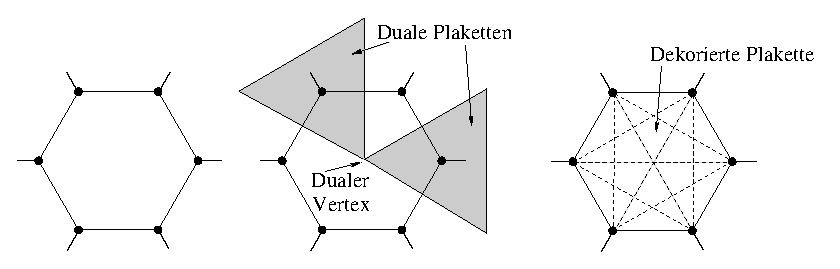
\includegraphics{./Euler-figs/decoratedtopo}
  \caption{Links ist eine Plakette des Sechseckgitters gezeigt. In der Mitte sind zwei duale Plaketten eingezeichnet, deren Vertices nicht benachbart sind. Diese Plaketten ber\"uhren sich am dualen Vertex des Sechseckes. Rechts ist das dekorierte Sechseck mit allen diagonalen Verbindungen dargestellt.  }
  \label{fig:decoratedtopo}
\end{figure}
Im Allgemeinen sind diese Vertices aber nicht benachbart, und die Muster, die entstehen, wenn duale Plaketten besetzt werden, haben nicht die Gittertopologie. Diese Zusammenhangsverh\"altnisse entsprechen einem Gitter, bei dem alle Vertices auf dem Rand einer Plakette miteinander verbunden sind. Ein solches Gitter heisst vollst\"andig dekoriertes Gitter.
In aller Regel wird Perkolation aber auf undekorierten Gittern behandelt. Die Euler-Charakteristik des undekorierten Gitters erh\"alt man \"uber den Umweg, statt den besetzten die unbesetzten Vertices mit dualen Plaketten zu belegen, und die Euler-Charakteristik des unbelegten Komplements zu berechnen (siehe Abb. \ref{fig:dualplaqu}). 
\begin{figure}[bp]
  \centering
  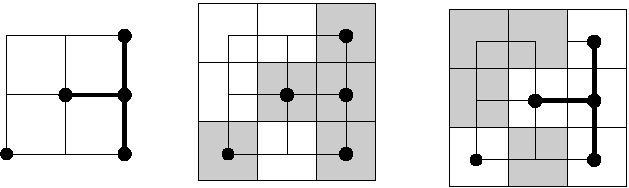
\includegraphics{./Euler-figs/dualplaqu}
  \caption{Links sind zwei Cluster auf dem Quadratgitter dargestellt. Setzt man auf jeden besetzten Vertex ein duales Quadrat (Mitte) entsteht eine zusammenh\"angende Figur. Besetzt man stattdessen die unbesetzten Vertices (rechts), zerf\"allt das Komplement in Komponenten, die den Clustern entsprechen. }
  \label{fig:dualplaqu}
\end{figure} 
Man berechnet zuerst $\chi(\bar{X})$ des Musters $\bar{X}$, das von den Plaketten auf unbesetzten Vertices gebildet wird. Die Vereinigung von $\bar{X}$ mit seinem Komplement $\check{X}$ ist die komplette Ebene, und die Summe der Euler-Charakteristiken von $\bar{X}$ und $\check{X}$ ist $1$ \cite{Saskin:89}. Die Euler-Charakteristik der offenen Menge $\check{X}$ ist daher $\chi(\check{X})=1-\chi(\bar{X})$. Wir wollen aber mit abgeschlossenen Mengen arbeiten und m\"ussen daher $\check{X}$ mit einem geeigneten Abschluss vereinigen. Der Rand $\partial \bar{X}$ von $\bar{X}$ ist ungeeignet, da er aus Kurven besteht, die sich selbst schneiden. Die Kurven w\"urden verschiedene Komponenten des Komplements miteinander verbinden und dadurch seine Zusammenhangsverh\"altnisse ver\"andern. Durch Modifikation der punktf\"ormigen \"Uberlappungen der Plaketten in $\bar{X}$, k\"onnen solche Kurven aber vermieden werden, ohne $\chi(\bar{X})$ zu ver\"andern (siehe Abb. \ref{fig:mod}).
\begin{figure}[htbp]
  \centering
  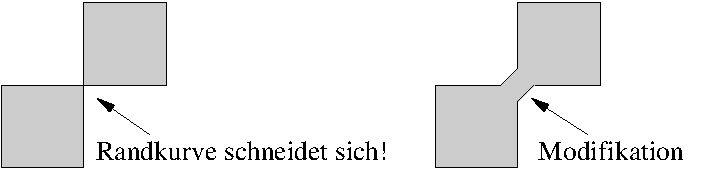
\includegraphics{./Euler-figs/mod}
  \caption{Notwendige Modifikation am Beispiel des Quadratgitters.}
  \label{fig:mod}
\end{figure}
Nachdem diese Modifikationen an $\bar{X}$ (und an $\check{X}$) durchgef\"uhrt worden sind, besteht der Rand $\partial \bar{X}$ nur noch aus geschlossenen einfachen Kurven, deren Euler-Charakteristik verschwindet. Die Euler-Charakteristik von $X=\check{X}\cup\partial \bar{X}$ ist also $\chi(X)=\chi(\check{X})=1-\chi(\bar{X})$.
\\Um die mittlere Euler-Charakteristik der Cluster, die durch Besetzten der Vertices eines undekorierten Gitters mit Wahrscheinlichkeit $p$ entstehen, zu berechnen, setzt man auf die Vertices eines Gitterausschnitts mit Wahrscheinlichkeit $q=1-p$ duale Plaketten und bestimmt die mittlere Euler-Charakteristik $\left<\chi(\bar{X})\right>_q$ dieser Muster $\bar{X}$. Die mittlere Euler-Charakteristik pro Vertex ist $\bar{\chi}(q):=\frac{1}{|V|}\left<\chi(\bar{X})\right>_q$, wobei $|V|$ die Zahl der Vertices im betrachteten Gitterausschnitt ist. Randterme verschwinden im Limes gro"ser Gitterausschnitte \cite{Jung:00}. F\"ur die Euler-Charakteristik des undekorierten Gitters erh\"alt man $\chi(p)=-\bar{\chi}(q)$; der Term $\frac{1}{|V|}$ verschwindet f\"ur $|V|\rightarrow \infty$. $\chi(p)$ und $\bar{\chi}(q)$ sind die Euler-Charakteristiken eines komplement\"ar besetzten Paares von matching-Gittern (siehe Abb. \ref{fig:chi}). Da die mittlere Euler-Charakteristik zweidimensionaler Gitter zwischen $0$ und $1$ nur eine Nullstelle hat \cite{Wagner:02}, ist die Nullstelle des self-matching Dreiecksgitters $p_0=\frac{1}{2}$ und f\"allt mit der Perkolationsschwelle zusammen. Die matching-Eigenschaft $\chi(p)=-\bar{\chi}(q)$ gilt nicht nur f\"ur planare Gitter, sondern auch f\"ur beliebige dekorierte Mosaike (siehe Abschnitt \ref{sec:matchingpoly}). F\"ur jedes self-matching Gitter gilt damit $p_0=p_c=\frac{1}{2}$. Wenn im Folgenden von der Euler-Charakteristik eines Gitters die Rede ist, sei die mittlere Euler-Charakteristik pro Vertex der Cluster verstanden, die beim Besetzen der Gittervertices mit Wahrscheinlichkeit $p$ entstehen. 
\begin{figure}[bp]
  \centering
  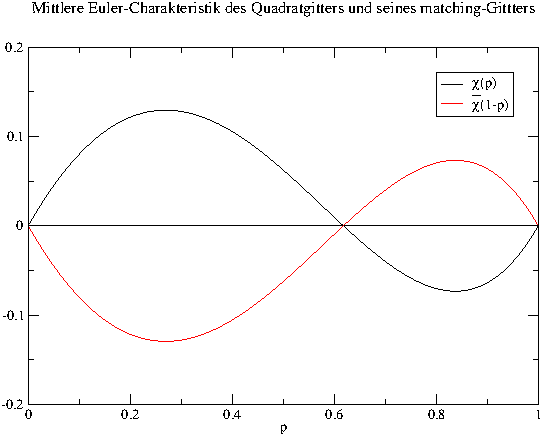
\includegraphics[width=10cm]{./Euler-figs/chi_fig}
  \caption{Mittlere Euler-Charakteristik des Quadratgitters und seines komplement\"ar besetzten matching-Gitters. Siehe Gleichung (\ref{eq:chisquare}).}
  \label{fig:chi}
\end{figure}
\\Am Beispiel des Quadratgitters mit Besetzungswahrscheinlichkeit $p$ soll hier die Berechnung von $\chi(p)$ mit den unterschiedlichen Methoden vorgef\"uhrt werden. Alle Gitterpl\"atze werden mit Wahrscheinlichkeit $q=1-p$ mit einem dualen Quadrat belegt. Wir berechnen also $\bar{\chi}(q)$ des mit Wahrscheinlichkeit $q$ besetzten matching-Gitters und erhalten durch $\chi(p)=-\bar{\chi}(1-p)$ die Euler-Charakteristik des Quadratgitters. Die Berechnung kann mit der Schnittrekursion oder durch Berechnung der Beitr\"age disjunkter randloser Zellen erfolgen.\\
Die \textbf{Schnittrekursion} ist mit jeder beliebig ausgerichteten Geradenschar $E_r$ m\"oglich. Die Euler-Charakteristiken der Schnitte mit den Geraden bezeichen wir mit $\chi^1(q)$. Zun\"achst w\"ahlen wir eine Schar $E_x$ parallel zu einer der Gitterrichtungen. Das Schnittmuster der Geraden mit den belegten Quadraten kann sich nur "andern, wenn die Gerade von einer Reihe Quadrate in die n\"achste wechselt (siehe Abb. \ref{fig:schnittquadrat}). Die kritischen Werte von $x$ liegen daher dort, wo duale Quadrate sich ber\"uhren.  
\begin{figure}[hbtp]
  \centering
  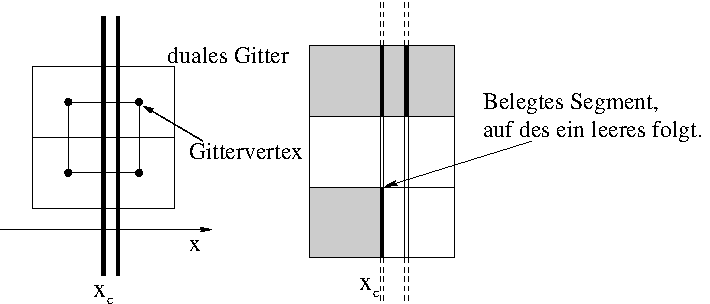
\includegraphics{./Euler-figs/schnittquadrat}
  \caption{Schnittrekursion beim Quadratgitter. Kritische Werte von $x$ liegen dort, wo sich duale Quadrate ber\"uhren. Im rechten Teil der Abbildung sind verschiedene Anordnungen und die resultierenden Schnittmuster auf den Geraden gezeigt.}
  \label{fig:schnittquadrat}
\end{figure}
\\Ein Segment der Geraden, also eine Kante des dualen Gitters, ist an kritschen Werten von $x=x_c$ belegt, wenn mindestens eines der angrenzenden Quadrate belegt ist. Die Zahl der Komponenten des Schnittmusters ist gleich der Zahl der belegten Segmente, auf die ein leeres Segment folgt. Die mittlere Euler-Charakteristik einer Gerade bei $x=x_c$, normiert auf die L\"ange, ist also $\chi^1_{x_c}(q)=(1-(1-q)^2)(1-q)^2$. Entsprechend ist f\"ur eine Gerade bei unkritischem $x$ die Euler-Charakteristik gleich $\chi^1_{x}=q(1-q)$. Die Differenz ergibt 
\begin{equation}
\label{eq:chisquare}
\bar{\chi}(q)=(1-(1-q)^2)(1-q)^2-(1-q)q=q-4q^2+4q^3-q^4,
\end{equation} 
und daher ist die mittlere Euler-Charakteristik des Quadratgitters $\chi(p)=-\bar{\chi}(1-p)=p-2p^2+p^4$.\\
Nun betrachten wir eine Schar von Geraden $E_r$, die zu keiner dualen Gitterkante parallel sind. Die Vertices des dualen Gitters entsprechen den kritischen Punkten und wir berechnen die erwartete \"Anderung von $\chi^1_{r_c}(q)$ in einer Umgebung des Vertex. In Abb. \ref{fig:morsequadrat} sind die einzigen beiden Konfigurationen gezeigt, bei denen sich $\chi^1_{r_c}(q)$ beim \"Uberstreichen des Vertex in Pfeilrichtung \"andert. Im ersten Fall betr\"agt die \"Anderung $-1$, und diese Konfiguration hat die Wahrscheinlichkeit $qp^3$. Im zweiten Fall ist die \"Anderung $+1$, und die Konfiguration hat Wahrscheinlichkeit $q^2p$. Es ergibt sich 
\begin{equation}
\bar{\chi}(q)=q(1-q)^3-q^2(1-q)=q-4q^2+4q^3-q^4
\end{equation} 
und damit $\chi(p)=-\bar{\chi}(1-p)=p-2p^2+p^4$.
Bei Verwendung dieser Geradenschar sieht man sehr gut, wie der Erwartungswert der Euler-Charakteristik durch lokale Beitr\"age der einzelnen Vertices zustande kommt, und wie sich unterschiedlichen Zusammenhangsverh\"altnisse des planaren und vollst\"andig dekorierten Gitters auf die Euler-Charakteristik auswirken.
\begin{figure}[hbtp]
  \centering
  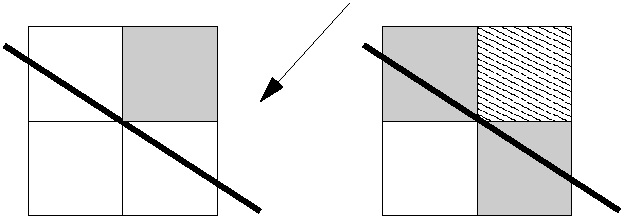
\includegraphics{./Euler-figs/morsequadrat}
  \caption{Die beiden Konfigurationen des Quadratgitters, die zur Schnittrekursion mit den eingezeichneten Geraden in Pfeilrichtung beitragen. Grau gezeichnete Quadrate sind besetzt, wei"se unbesetzt. Die linke Konfiguration hat Wahrscheinlichkeit $q(1-q)^3$ und tr\"agt $+1$ bei, die rechte hat Wahrscheinlichkeit $q^2(1-q)$ und tr\"agt $-1$ bei. Der Zustand des schraffierten Quadrates ist f\"ur die \"Anderung von $\chi^1_{r_c}(q)$ unerheblich.}
  \label{fig:morsequadrat}
\end{figure}
\\Eine andere, h\"aufig zweckm\"a"sigere, Methode, die Mittelwerte auszurechnen, besteht darin, das duale Gitter in \textbf{disjunkte Zellen} zu zerlegen und die erwartete Anzahl derjenigen Zellen zu bestimmen, die durch Belegen mit dualen Plaketten bedeckt werden \cite{Likos:95}. Die disjunkten Zellen sind die Plaketten ohne Rand, die Kanten ohne Endpunkte und die Vertices des dualen Gitters. 
\begin{itemize}
\item Plaketten sind mit Wahrscheinlichkeit $q$ belegt und auf ihre Gesamtzahl $|V|$ wird normiert. 
\item Duale Kanten sind bedeckt, wenn mindestens eine der angrenzenden Plaketten belegt ist; die Wahrscheinlichkeit daf\"ur ist $(1-(1-q)^2)=1-p^2$. Jede duale Kante entspricht einer Kante des urspr\"unglichen Gitters. Daher ist die Zahl der dualen Kanten pro dualer Plakette gleich der Zahl der Kanten pro Vertex. Sie betr\"agt $\frac{z}{2}$, denn jede Kante endet an 2 Vertices, und von jedem Vertex gehen $z$ Kanten aus.
\item Ein dualer Vertex ist in allen $n$ umgebenden dualen Plaketten enthalten und daher mit Wahrscheinlichkeit $(1-(1-q)^n)=1-p^n$ pr\"asent. $n$ ist die Kantenzahl der Plakette des urspr\"unglichen Gitters, in der der duale Vertex sitzt.
\end{itemize}
F\"ur das Quadratgitter ist $z=4$ und die Zahl der Quadrate ist gleich der Zahl der Vertices. Man erh\"alt wie oben 
\begin{equation}
\bar{\chi}(q)=q-2(1-(1-q)^2)+(1-(1-q)^4)=q-4q^2+4q^3-q^4
\end{equation} 
und damit $\chi(p)=p-2p^2+p^4$.\\

Die mittlere Koordinationszahl eines Gitters ist \"uber den Euler'schen Satz durch die Zahl der Plaketten bestimmt, und alle Kanten sind bei Besetzung der dualen Plaketten mit der gleichen Wahrscheinlichkeit $1-p^2$ vorhanden. Daher h\"angt die mittlere Euler-Charakteristik eines planaren zweidimensionalen Gitter ausschlie"slich von der Anzahl seiner Plaketten und deren Kantenzahl ab.\\

\subsubsection{Gittertiere}
In zwei Dimensionen ist die Euler-Charakteristik einer Gitterkonfiguration die Differenz der Anzahl der Cluster und der Anzahl der L\"ocher in diesen Clustern. Nach Konstruktion ist jedes Loch ein Cluster des komplement\"ar besetzten matching-Gitters. Die Zahl der Cluster pro Vertex auf dem mit Wahrscheinlichkeit $p$ besetzten Gitter ist $n(p)$; die Zahl Cluster pro Vertex des mit Wahrscheinlichkeit $q=1-p$ besetzten matching-Gitter ist $n^*(q)$. Die mittlere Euler-Charakteristik des Gitters ist also die Differenz von $n(p)$ und $n^*(q)$. Im Abschnitt \ref{sec:animals} wurde die Zahl der Cluster pro Vertex durch eine Summe \"uber alle m\"oglichen endlichen Cluster, die sog. Gittertiere oder lattice animals, ausgedr\"uckt. Mit den Anzahlen der m\"oglichen Cluster $g_{st}$ bzw. $g^*_{st}$ der Masse $s$ und Umfang $t$ auf den beiden Gittern erh\"alt man 
\begin{equation}
n(p)=\sum_{s,t}g_{st}p^sq^t \qquad \text{und} \qquad n^*(q)=\sum_{s,t}g^*_{st}q^sp^t.
\end{equation}  
Der unendliche Cluster spielt hier keine Rolle, denn der Beitrag eines einzigen Clusters zur Zahl der Cluster pro Vertex verschwindet. 
Die mittlere Euler-Charakteristik ist damit
\begin{equation}
  \label{eq:chianimals}
  \chi(p)=\sum_{s,t} \left(g_{st}p^sq^t-g^*_{st}q^sp^t\right).
\end{equation}
Die ersten Cluster, die zu diesen Reihen beitragen, sind f\"ur den Fall des Quadratgitters in Abbildung \ref{fig:animals} dargestellt. Die $\chi(p)$ ist also die Differenz zweier unendlicher Polynome. Andererseits l\"asst sich $\chi(p)$ lokal ausrechnen und ist ein Polynom endlicher (kleiner) Ordnung. Die Terme in Gl. (\ref{eq:chianimals}) m\"ussen sich also bis auf einige wenige wegheben \cite{Sykes:64}.
\begin{figure}[tbp]
  \centering
  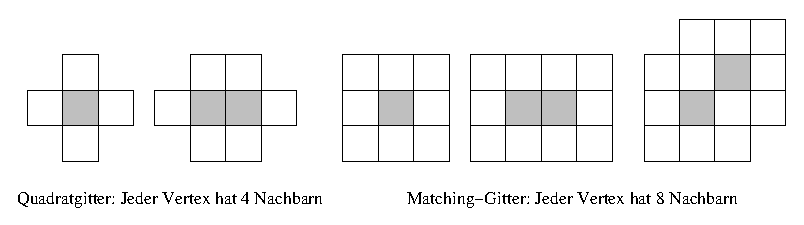
\includegraphics{./Euler-figs/animals}
  \caption{Gittertiere bis zur Gr\"o"se $s=2$ auf dem Quadratgitter (links) und auf dem machting-Gitter (rechts) mit $t=4$ und $t=6$ bzw. $t=8$, $t=10$ und $t=12$. Es ist jeweils nur eine Orientierung der Gittertiere dargestellt.}
  \label{fig:animals}
\end{figure}
Die Zahl $g_{st}$ steigt mit $s$ und $t$ schnell an, und wurde f\"ur das Quadratgitter bis $s = 22$ und $t=46$ von Mertens \cite{Mertens:90} mit Hilfe von Computern abgez\"ahlt. 
Auf dem Quadratgitter kommen die Terme, die zu $\chi(p)$ beitragen, ausschlie"slich von $n(p)$, da $n^*(q)$ als Polynom in $p$ erst mit $p^8$ beginnt:
\begin{equation}
  \begin{split}
  \chi(p)&=pq^4+2p^2q^6+p^3(4q^6+2q^7)+p^4(9q^8+8q^9+2q^{10})+\cdots\\
&-qp^8-q^2(2p^{10}+2p^{12})-\cdots\\
 &=p-2p^2+p^4.
  \end{split}
\end{equation}


\subsubsection{Euler-Charakteristik dekorierter Mosaike}
\label{sec:matchingpoly}
Fortuin und Kastelyn haben 1972 in einer Serie von Arbeiten \cite{Fortuin:72} das Random-Cluster-Modell vorgestellt und gezeigt, dass bond-Perkolation dem Limes $\lambda \rightarrow 1$ eines Potts-Modells, dessen Spins $\lambda$ verschiedene Zust\"ande annehmen k\"onnen, entspricht. Essam \cite{Essam:79} hat diese Korrespondenz durch Einf\"uhrung von Wechselwirkungen, an denen mehrere Spins teilnehmen, auf site-Perkolation erweitert. Die Dualit\"at der Hoch- und Tieftemperaturzustandssumme zweidimensionaler Pottsmodelle entspricht im Limes $\lambda \rightarrow 1$ der matching-Eigenschaft der site-Perkolation. Das matching-Polynom, das Essam einf\"uhrt, ist die mittlere Euler-Charakteristik des assoziierten Perkolationsproblems. Der Wechselwirkungsgraph des Pottsmodells aus \cite{Essam:79} l\"asst sich f\"ur jedes dekorierte Mosaik konstruieren, so dass die mittlere Euler-Charakteristik eines site-Perkolationsproblems auf beliebig dekorierten Mosaiken berechnet werden kann. Die folgende Konstruktion ist so zu verstehen, dass sie zun\"achst auf einem endlichen Gitterausschnitt durchgef\"uhrt wird. Anschlie"send muss der Limes zu unendlichen Gittern in geeigneter Weise durchgef\"uhrt werden \cite{Essam:79}. \\
Der Wechselwirkungsgraph setzt sich aus Spinvertices $s\in S$ und Wechselwirkungsvertices $i\in I$ zusammen. Um den Wechselwirkungsgraph eines Perkolationsproblems auf einem dekorierten Mosaik zu erhalten, werden Spins auf alle Kanten und in alle dekorierten Plaketten des Mosaiks gesetzt. Die Wechselwirkungsvertices sitzen auf den Ecken des Mosaiks (siehe Abb. \ref{fig:interactiongraph}).
\begin{figure}[tbp]
  \centering
  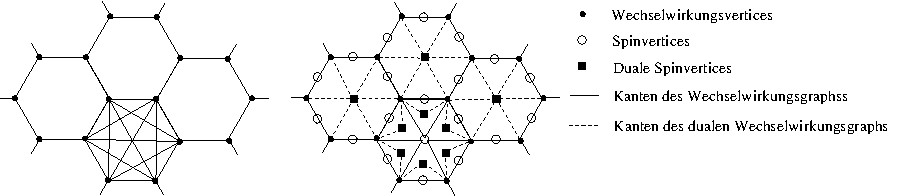
\includegraphics{./Euler-figs/interactiongraph}
  \caption{Ausschnitt aus einem dekorierten Mosaik (links) und die resultierenden Wechselwirkungsgraphen (rechts).}
  \label{fig:interactiongraph}
\end{figure}
Ein Wechselwirkungsvertex $i$ vermittelt eine Wechselwirkung zwischen allen Spins auf den Kanten und in den Plaketten, die diesen Vertex umgeben. Jeder Wechselwirkungsvertex $i$ wird mit allen Spinvertices verbunden, die in $i$ wechselwirken. Dadurch entsteht ein bipartiter, planarer und zusammenh\"angender Graph $G$. Zu diesem Graphen wird ein ein dualer Wechselwirkungsgraph $G^*$ konstruiert, dessen Vertexmenge aus dualen Spinvertices $s^* \in S^*$ und den Wechselwirkungsvertices $i\in I$ besteht. Die dualen Spinvertices $s^* \in S^*$ werden in alle Plaketten von $G$ gesetzt, und jeder Wechselwirkungsvertices wird mit allen umgebenden dualen Spins verbunden (siehe Abb. \ref{fig:interactiongraph}).
\\Wir betrachten nun den Subgraph $G=(V,E)$ mit Vertexmenge $V=S\cup I'$, $I'\subset I$, und den Subgraph $G^*=(V^*,E^*)$ mit Vertexmenge $V^*=S^*\cup I\backslash I'$. Die Kantenmengen der Subgraphen bestehen aus allen Kanten, deren Endvertices beide in $V$ bzw. $V^*$ sind. Bettet man beide Graphen in die Ebene ein, ist jede endliche Komponente von $G$ in einer Plakette von $G^*$ enthalten; gleiches gilt umgekehrt \cite{Essam:79}. Die Differenz der Komponenten $n(G)$ und $n^*(G^*)$ von $G$ bzw. $G^*$ ist nach dem Euler'schen Satz 
\begin{equation}
  n(G)-n^*(G^*)=|V|-|E|-1
\end{equation}
Der Term $-1$ entspricht der unendlichen Komponente. W\"ahlt man Vertices $I'$ aus $I$ mit Wahrscheinlichkeit $p$ aus und mittelt \"uber alle Konfigurationen, erh\"alt man die mittlere Euler-Charakteristik. Komponenten, die nur aus isolierten Spins bestehen, entsprechen keinen Clustern oder L\"ochern des Perkolationsproblems auf dem dekorierten Mosaik und m\"ussen daher noch abgezogen werden (Summen \"uber $S$ und $S^*$ in Gl. (\ref{eq:matchingpoly})). Das Resultat ist das matching-Polynom \cite{Essam:79} oder die mittlere Euler-Charakteristik:
\begin{equation}
  \chi(p)=|S|+\sum_{i\in I} p-\sum_{i\in I} z_i p-1 -\sum_{s \in S}(1-p)^{z_s}+\sum_{s^* \in S^*}p^{z_{s^*}}.
  \label{eq:matchingpoly}
\end{equation}
$z_v$ ist die Koordinationszahl des Vertex $v$. Um $\chi(p)$ zu normieren, muss noch durch $|I|$ geteilt werden. Da $G$ ein zusammenh\"angender Graph ist, gilt nach dem Euler'schen Satz $v-e+f=|S|+|I|-\sum_{i\in I}z_i +|S^*|=2$ (die unendliche Plakette mitgez\"ahlt) und damit die matching-Relation $\chi(p)=-\chi^*(1-p)$ f\"ur beliebige komplement\"ar dekorierte Mosaike.
\\F\"ur planare und vollst\"andig dekorierte Gitter stimmen die mit Gleichung (\ref{eq:matchingpoly}) berechneten Euler-Charakteristiken mit den Ergebnissen, die mit den anderen Methoden erhalten werden, \"uberein. Man \"uberzeugt sich leicht, dass die einzelnen Terme aus (\ref{eq:matchingpoly}) in diesen F\"allen den Beitr\"agen der Plaketten, Kanten und Ecken entsprechen. 

\subsection{Dreidimensionale Gitter}
Im vorigen Abschnitt haben wir gesehen, dass die Vereinigung dualer Zellen eines zweidimensionalen Gitters die topologischen Eigenschaften des vollst\"andig dekorierten Gitters hat. Das Komplement hat die Zusammenhangsverh\"altnisse des undekorierten Gitters.\\
Entsprechendes gilt unter bestimmten Voraussetzungen f\"ur dreidimensionale Gitter. Wir betrachten ein Gitter und raumf\"ullende Zellen um die Vertices, z.B. W\"urfel um die Vertices des einfach-kubischen Gitters (sc-Gitter). Die Vereinigung dieser Zellen hat die topologischen Eigenschaften eines Gitters, dessen Vertices miteinander verbunden sind, wenn ihre Zellen einen nichtleeren Durchschnitt haben. Beim sc-Gitter sind das alle W\"urfel, die eine Ecke, Kante oder Fl\"ache teilen, und jeder Vertex h\"atte 26 Nachbarn. Vertices des Gitter haben aber in der Regel sehr viel weniger Nachbarn; das sc-Gitter beispielweise nur sechs. Wenn die und nur die Zellen, deren Vertices Gitternachbarn sind, einen Durchschnitt haben der nur in diesen beiden Zellen enthalten ist, hat das Komplement die topologischen Eigenschaften des Gitters. Das sc-Gitter erf\"ullt diese Voraussetzung, denn Kanten sind in vier und Ecken in acht W\"urfeln enthalten, w\"ahrend die Fl\"achen nur zu zwei W\"urfeln geh\"oren und den Gitterkanten entsprechen. 
\\Um zu einem Vertex eine Zelle zu konstruieren, betrachtet man die Ebenen senkrecht auf der Mitte der Verbindungslinien zu den n\"achsten, \"ubern\"achsten, usw. Gitternachbarn. Jede dieser Ebenen definiert einen Halbraum, der den Vertex enth\"alt. Die Wigner-Seitz-Zelle (WSZ) eines Gittervertex ist der Durchschnitt aller so konstruierten Halbr\"aume. Die WSZ der Bravais-Gitter sind raumf\"ullend. Wenn jede Fl\"ache der WSZ einer Gitterkante entspricht und die WSZ raumf\"ullend sind, sind die WSZ geeignet, um die Euler-Charakteristik zu bestimmen. Bei manchen Gittern, z.B. dem bcc-Gitter, haben die WSZ aber mehr Fl\"achen als Gitternachbarn.
\\F\"ur Gitter, die keine Bravaisgitter sind, oder deren WSZ zu viele Fl\"achen haben, kann man dennoch geeignete raumf\"ullende Zellen finden. Diese sind aber h\"aufig nicht konvex. Der Durchschnitt zweier Gitternachbarn besteht dann aus verschiedenen Fl\"achenst\"ucken, inklusive den zwischen diesen St\"ucken liegenden Kanten (siehe Abb. \ref{fig:bcc_nonconvex_app}). 
\\Ob der Durchschnitt der Gitternachbarn eben ist oder nicht, spielt keine Rolle; wichtig ist nur, dass der Durchschnitt der Zellen zweier Gitternachbarn, abgesehen von den Randkanten, nur in diesen Zellen enthalten ist, und dass der Durchschnitt aller \"ubrigen Zellen in mehr als zwei Zellen enthalten ist. Dadurch wird gew\"ahrleistet, dass unbesetzte Zellen, die keine Gitternachbarn sind, durch besetzte Zellen getrennt werden, und dass eben dies bei Gitternachbarn nicht geschieht.
\\Hat man geeignete Zellen gefunden, werden die Zellen, die unbesetzten Vertices entsprechen, ausgew\"ahlt, und die Euler-Charakteristik der entstehenden Figur $\bar{X}$ ausgerechnet. Die Euler-Charakteristik des Komplements $\check{X}$ ist $\chi(\check{X})=-\chi(\bar{X})+\mathcal{O}(1)$; $\check{X}$ ist aber eine offene Menge. Damit der Rand $\partial \bar{X}$ ein geeigneter Abschluss von $\check{X}$ ist, muss im dreidimensionalen Fall $\bar{X}$ \"uberall dort modifiziert werden, wo Zellen nur an Ecken oder Kanten \"uberlappen. Die Euler-Charakteristik $\chi(\bar{X})$ bleibt bei diesen Modifikationen unver\"andert. Die Euler-Charakteristik des Randes nach der Modifikation ist nach Gleichung (\ref{eq:opensets}) $\chi(\partial \bar{X})=2\chi(\bar{X})$. Damit erh\"alt man f\"ur der Euler-Charakteristik der Vereinigung $X$ von $\check{X}$ (entsprechend modifiziert) mit $\partial \bar{X}$ 
\begin{equation}
  \chi(X)=\chi(\check{X})+\chi(\partial \bar{X})=-\chi(\bar{X})+2\chi(\bar{X})+\mathcal{O}(1)=\chi(\bar{X})+\mathcal{O}(1)
\end{equation}
Uns interessiert hier die mittlere Euler-Charakteristik pro Vertex $\chi(p)$ der Muster, die bei site-Perkolation mit Besetzungswahrscheinlichkeit $p$ entstehen. Die Euler-Charakteristik $\chi(p)$ ist gleich der des Komplements $\bar{\chi}(1-p)$. Wie in zwei Dimensionen verschwinden m\"ogliche Randterme im Limes gro"ser Gitter \cite{Jung:00}. Am Beispiel des sc-Gitter werden zwei Methoden, $\chi(p)$ zuberechnen, vorgestellt.
\\Die mittlere Euler-Charakteristik des sc-Gitters l\"asst sich einfach mit der \textbf{Schnittrekursion} und einem Satz von Ebenen, die parallel zu den Gitterebenen sind, bestimmen. Das Schnittmuster der Ebene mit den besetzten W\"urfeln, ist ein Muster aus Quadraten eines Quadratgitters. Die Muster \"andern sich, wenn die Ebene von einer Schicht W\"urfel in die n\"achste wandert. Zwischen zwei Schichten von W\"urfeln sind die Quadrate des Schnittmusters belegt, wenn mindestens einer der angrenzenden W\"urfel besetzt ist. Das Schnittmuster hat daher die Euler-Charakteristik eines mit Wahrscheinlichkeit $1-(1-q)^2$ besetzten, vollst\"andig dekorierten Quadratgitters $\bar{\chi}^{Qu}(1-(1-q)^2)$. Schnittmuster der Ebenen, die nicht zwischen zwei Schichten von W\"urfeln liegen sind entsprechend mit Wahrscheinlichkeit $q$ belegt und haben Euler-Charakteristik $\bar{\chi}^{Qu}(q)$. Ihre Differenz ist die Euler-Charakteristik des einfach-kubischen Gitters
\begin{equation}
\begin{split}
  \chi(p) & =\bar{\chi}(1-p)=\bar{\chi}^{Qu}(1-p^2)-\bar{\chi}^{Qu}(1-p)\\
&=p-3p^2+3p^4-p^8.
\end{split}
\end{equation}
\\Wenn ein Gitter keine einfache Schichtstruktur vorgibt, ist es zweckm\"a"siger $\bar{\chi}(q)$ aus den Beitr\"agen \textbf{disjunkter Zellen} zu berechnen \cite{Likos:95}. Dazu m\"ussen die Wahrscheinlichkeiten, dass die unterschiedlichen Zellen zur Figur geh\"oren, wenn abgeschlossene W\"urfel mit Wahrscheinlichkeit $q=1-p$ ausgew\"ahlt werden, bestimmt werden. 
\begin{itemize}
\item \textbf{W\"urfel} sind mit Wahrscheinlichkeit $q$ vorhanden. Jeder besetzte W\"urfel tr\"agt $-1$ bei.
\item Damit eine \textbf{Fl\"ache} zur Anordnung geh\"ort, muss mindestens einer der angrenzenden W\"urfel besetzt sein. Jede Fl\"ache ist also mit Wahrscheinlichkeit $1-(1-q)^2=1-p^2$ vorhanden. Ein W\"urfel hat sechs Fl\"achen, die je zu zwei W\"urfeln geh\"oren. Es gibt daher drei Fl\"achen pro W\"urfel, die $+1$ beitragen, wenn mindestens einer der angrenzenden W\"urfel besetzt ist.
\item Eine \textbf{Kante} ist Teil von vier W\"urfeln und daher mit Wahrscheinlichkeit $1-p^4$ pr\"asent. Ein W\"urfel hat zw\"olf Kanten, die aber je in vier W\"urfeln enthalten sind, und folglich gibt es drei Kanten pro W\"urfel. Eine Kante tr\"agt $-1$ zur Euler-Charakteristik bei.
\item Die \textbf{Ecke} eines W\"urfels ist auch Ecke von sieben anderen W\"urfeln und daher mit Wahrscheinlichkeit $1-p^8$ vorhanden. Pro W\"urfel gibt es eine Ecke, die, wen sie Teil der Anordnung ist, $+1$ beitr\"agt.
\end{itemize}
Summation der Beitr\"age liefert $\bar{\chi}(q)$ und damit auch $\chi(p)$:
\begin{equation}
  \chi(p)  =\bar{\chi}(1-p)=-(1-p)+3(1-p^2)-3(1-p^4)+1-p^8=p-3p^2+3p^4-p^8.
\end{equation}\\

Die Wahl der Zellen zur Berechnung der Euler-Charakteristik eines Gitters ist im Allgemeinen nicht eindeutig. Daher werden zur Unterscheidung unterschiedlicher Euler-Charakteristiken neben dem Namen des Gitters auch die Zahl $z$ der Fl\"achen einer Zelle, d.h. die Zahl der Gitternachbarn eines Vertex, und die Zahl $\bar{z}$ der Zellen, mit denen eine gegebene Zellen einen nichtleeren Durchschnitt hat, angegeben. Die Zahl $\bar{z}$ ist die Koordinationszahl eines Gitters, dessen Vertices verbunden sind, wenn die zugeh\"origen Zellen einen nichtleeren Durchschnitt haben. Dieses Gitter ist das Analogon eines vollst\"andig dekorierten Gitters in zwei Dimensionen. Anders als in zwei Dimensionen h\"angt es aber von der Wahl der Zellen ab. 
\\Ein Vertex des sc-Gitters hat sechs Nachbarn, und ein W\"urfel teilt mit 26 W\"urfeln eine Fl\"ache, Kante oder Ecke. F\"ur die mittlere Euler-Charakteristik des sc-Gitter schreiben wir somit $\chi^{sc}_{6-26}(p)$.
\\Die Berechnung der Euler-Charakteristik anderer Gitter und Gitter h\"oherer Dimensionen geht analog, ist aber h\"aufig um vieles aufwendiger.

